\begin{figure}[H]
    \centering
    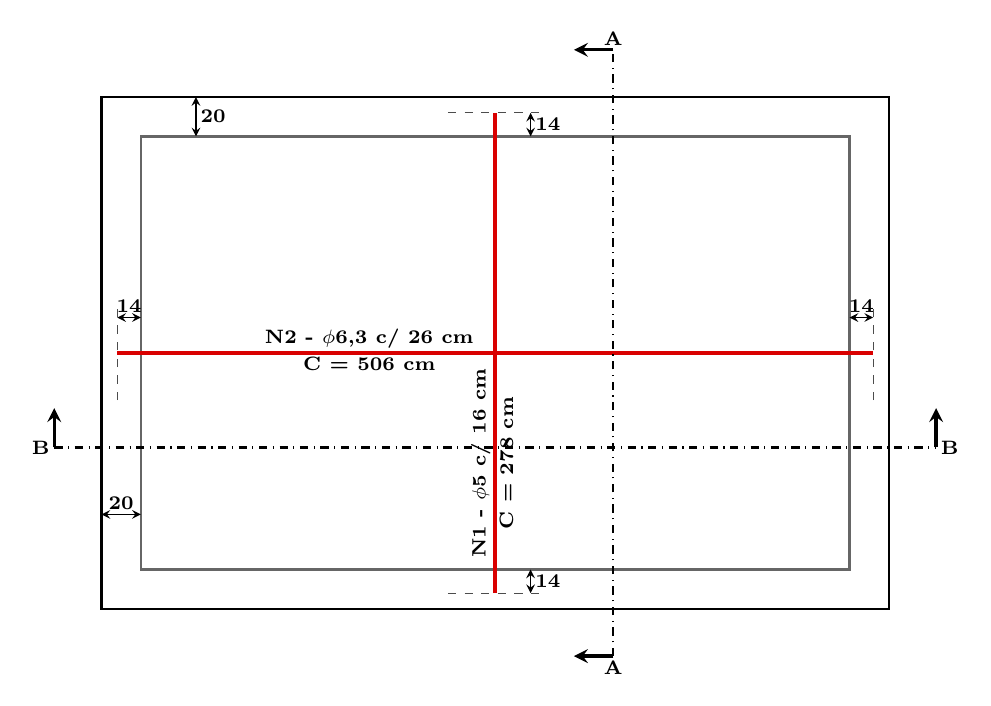
\begin{tikzpicture}[
        scale=1,
        >=stealth,
        contorno/.style={draw=black, thick},
        margem/.style={draw=gray!80!black, thick},
        barra/.style={line width=1.6pt, red!85!black},
        chamada/.style={gray!60!black, thin, dashed},
        cota/.style={<->, thin, black},
        corte/.style={draw=black, dash dot, thick},
        setaCorte/.style={->, very thick, black},
        txt/.style={font=\scriptsize\bfseries, inner sep=1.5pt}
    ]

    % ---------- Parâmetros (planta) ----------
    \def\W{10}      % largura do retângulo maior
    \def\H{6.5}     % altura do retângulo maior (menor que \W)
    \def\m{0.5}     % distância entre os retângulos (= 20 em x e y)
    \def\ext{0.3}   % quanto a barra sai do retângulo menor (< \m)
    \pgfmathsetmacro\cx{\W/2}
    \pgfmathsetmacro\cy{\H/2}
    \pgfmathsetmacro\xa{\cx+1.5}   % posição do corte AA (vertical)
    \pgfmathsetmacro\yb{\cy-1.2}   % posição do corte BB (horizontal)

    % ========== 1. VISTA EM PLANTA ==========
    \draw[contorno] (0,0) rectangle (\W,\H);
    \draw[margem]   (\m,\m) rectangle (\W-\m,\H-\m);

    % Cota da margem (20)
    \draw[cota] (1.2,\H-\m) -- (1.2,\H) node[midway, right, txt] {20};
    \draw[cota] (\m,1.2) -- (0,1.2) node[midway, above, txt] {20};

    % Barra horizontal (principal)
    \draw[barra] (\m-\ext,\cy) -- (\W-\m+\ext,\cy);
    % Barra vertical (secundária)
    \draw[barra] (\cx,\m-\ext) -- (\cx,\H-\m+\ext);

    % Linhas tracejadas nas pontas + cotas em relação ao retângulo menor
    \foreach \xp/\xi in {\m-\ext/\m, \W-\m+\ext/\W-\m} {
        \draw[chamada] (\xp,\cy-0.6) -- (\xp,\cy+0.6);
        \draw[cota] (\xp,\cy+0.45) -- (\xi,\cy+0.45)
            node[midway, above, txt] {14};
    }
    \foreach \yp/\yi in {\m-\ext/\m, \H-\m+\ext/\H-\m} {
        \draw[chamada] (\cx-0.6,\yp) -- (\cx+0.6,\yp);
        \draw[cota] (\cx+0.45,\yp) -- (\cx+0.45,\yi)
            node[midway, right, txt] {14};
    }

    % Valores em cima e em baixo das barras
    \node[txt, above] at (\cx-1.6,\cy) {N2 - $\phi$6,3 c/ 26 cm};
    \node[txt, below] at (\cx-1.6,\cy) {C = 506 cm};
    \node[txt, above, rotate=90] at (\cx,\cy+1.4) {};
    \node[txt, rotate=90, above] at (\cx,\cy-1.4) {N1 - $\phi$5 c/ 16 cm};
    \node[txt, rotate=90, below] at (\cx,\cy-1.4) {C = 278 cm};

    % Cortes AA (vertical) e BB (horizontal)
    \draw[corte] (\xa,-0.6) -- (\xa,\H+0.6);
    \draw[setaCorte] (\xa,\H+0.6) -- ++(-0.5,0);
    \draw[setaCorte] (\xa,-0.6)   -- ++(-0.5,0);
    \node[txt, above] at (\xa,\H+0.6) {A};
    \node[txt, below] at (\xa,-0.6)   {A};

    \draw[corte] (-0.6,\yb) -- (\W+0.6,\yb);
    \draw[setaCorte] (-0.6,\yb)   -- ++(0,0.5);
    \draw[setaCorte] (\W+0.6,\yb) -- ++(0,0.5);
    \node[txt, left]  at (-0.6,\yb)   {B};
    \node[txt, right] at (\W+0.6,\yb) {B};

    %\node[txt] at (\cx,-1.2) {PLANTA DA LAJE};

    \end{tikzpicture}
    %\caption{Planta da laje e cortes AA e BB}
\end{figure}